\documentclass[9pt,twocolumn]{confpaper}

%%%%%%%%%%%%%%%%%%%%  INCLUDES  %%%%%%%%%%%%%%%%%%%%%%%%%%

%%%%%%%%%%%%%%%%%%%%  LOCALS  %%%%%%%%%%%%%%%%%%%%%%%%%%%%

\newcommand{\system}{{\em NetASM}}

%%%%%%%%%%%%%%%%%%%%  TITLE/AUTHORS  %%%%%%%%%%%%%%%%%%%%%

\date{}
\title{\ttlfnt{
Alternative Trust Sources:\\ Reducing DNSSEC Signature Verification Operations \\with TLS}}
\author{
  \aufnt{Sean Donovan} \\
  \affaddr{Georgia Institute of Technology}
  \and
  \aufnt{Nick Feamster} \\
  \affaddr{Princeton University}
}

%%%%%%%%%%%%%%%%%%%%  START OF DOCUMENT  %%%%%%%%%%%%%%%%%

\begin{document}

\maketitle

%\setcopyright{rightsretained} 
%\conferenceinfo{SIGCOMM '15}{August 17-21, 2015, London, United Kingdom} 
%\isbn{978-1-4503-3542-3/15/08}
%\doi{http://dx.doi.org/10.1145/2785956.2790001}

\AcmCopyright
%\ToAppear

\begin{sloppypar}

\begin{abstract}
DNSSEC has been in development for 20 years. It provides for provable security
when retrieving domain names through the use of a public key infrastructure 
(PKI). Unfortunately, there is also significant overhead involved with DNSSEC:
verifying certificate chains of signed DNS messages involves extra computation,
queries to remote resolvers, additional transfers, and introduces added latency
into the DNS query path.
We pose the question: is it possible to achieve practical security without 
always verifying this certificate chain if we use a different, outside source of
trust between resolvers?
We believe we can. 
Namely, by using a long-lived, mutually authenticated
TLS connection between pairs of DNS resolvers, we suggest that we can maintain 
near-equivalent levels of security with very little extra overhead compared to a
non-DNSSEC enabled resolver. 
By using a reputation system or probabilistically verifying a portion of DNSSEC
responses would allow for near-equivalent levels of security to be reached, even
in the face of compromised resolvers.

\end{abstract}


\ifthenelse{\equal{\onlyAbstract}{no}}{% !onlyAbstract

\section{Introduction}\label{sec:intro}

DNSSEC is not a new technology; it has been in development since 1995, with the
first RFC published in 1997.\cite{dnssecHistory} Unfortunately, deployment 
has been slow but incremental due to, among other reasons, significant 
infrastructure investments needed to handle the overhead costs
required to verify DNSSEC responses.

DNSSEC requires verification of a certificate signature chain in order to 
maintain security. There are fourfold costs. First are calculating the 
signatures. Fortunately, this cost is getting cheaper due to processor 
improvements and is not the focus of this paper. Second are the additional DNS 
query costs. In order to verify signatures, DNS resolvers must request 
additional signature-related DNS records from various servers on the certificate
chain.
Third are the additional bandwidth costs. There are additional DNSSEC-specific 
records contributing, but the extra queries are a bulk of the extra bandwidth 
needs.
In one study, these two costs were estimated such that 
resolvers would need to be sized to ``handle 10 times the query volume ... and a
total response traffic volume of 100 times greater.''\cite{huston2013} 
Finally, there are the latency costs for end hosts as the verification 
activities take  non-trivial time.

These costs are significant, especially regarding equipment provisioning. We 
seek to reduce these costs by relying on an \emph{outside source of trust} in
place of signature verification. 
By using a different way of finding trust between DNSSEC-enabled resolvers, we 
can cut down on the amount of PKI verifications and further queries that are 
necessary for traditional DNSSEC. 

\begin{figure}
  \centering
  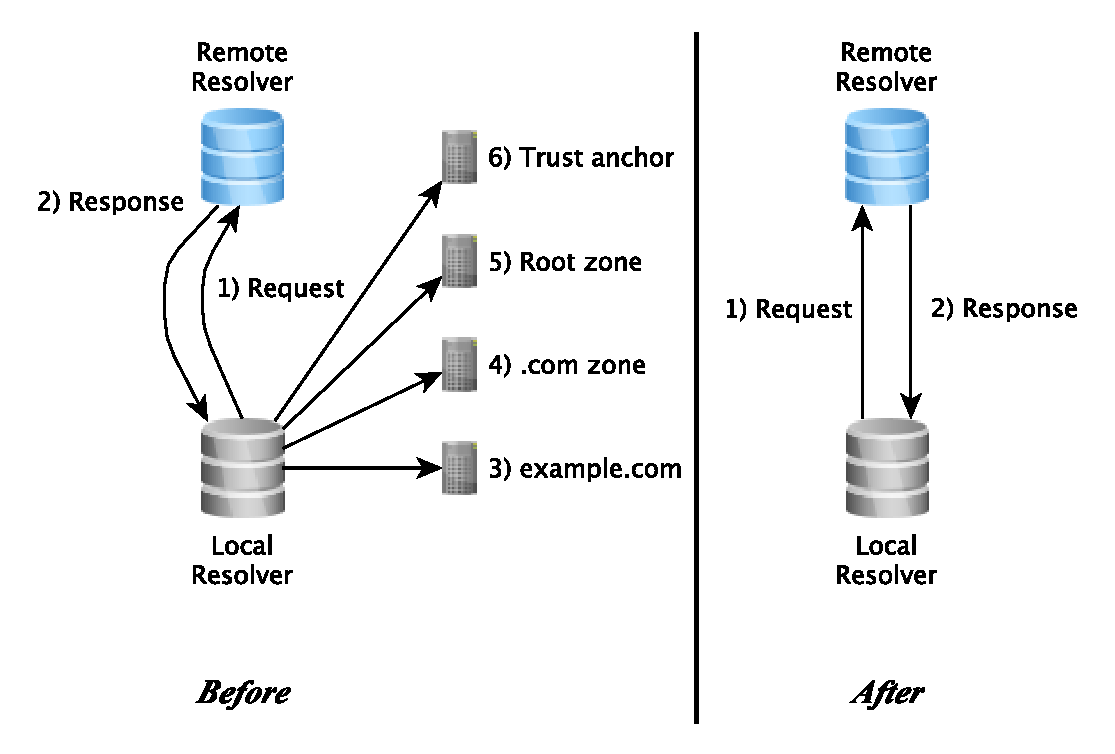
\includegraphics[width=1.0\columnwidth]{figures/before-and-after}
  \caption{Before, to verify the certificate chain that DNSSEC relies upon, many further requests are necessary to verify signatures. With our proposal, there is a long-lived, mutually authenticated TLS connection between both resolvers that the requests and responses travel across. If the local resolver knows who is at the other end of the connection, and it trusts that the remote resolver has verified signatures, the local resolver should not need to verify the same signatures itself.}
  \label{fig:before-and-after}
\end{figure}


%\begin{figure}
%  \begin{minipage}{\textwidth}
%  \begin{minipage}{\columnwidth}
%    \begin{subfigure}{.5\columnwidth}
%      \centering
%      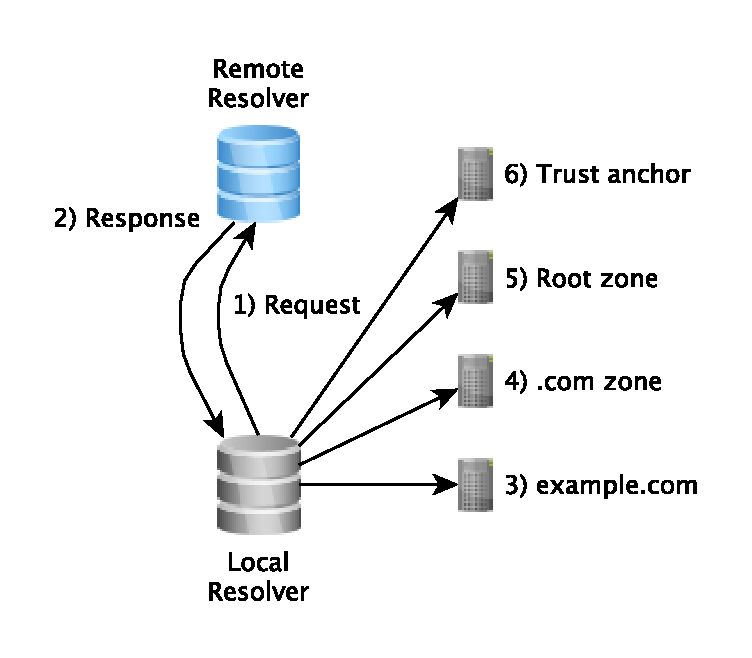
\includegraphics[width=1.0\columnwidth]{figures/before}
%      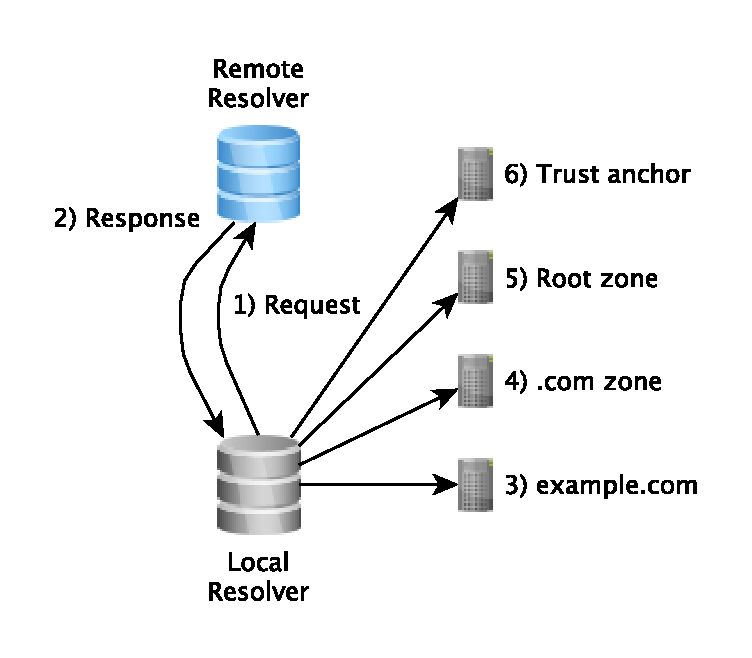
\includegraphics[width=.8\columnwidth]{figures/before}
%      \caption{\textbf{Before}}
%      \label{fig:before}
%    \end{subfigure}
%    \begin{subfigure}{.5\columnwidth}
%      \centering
%      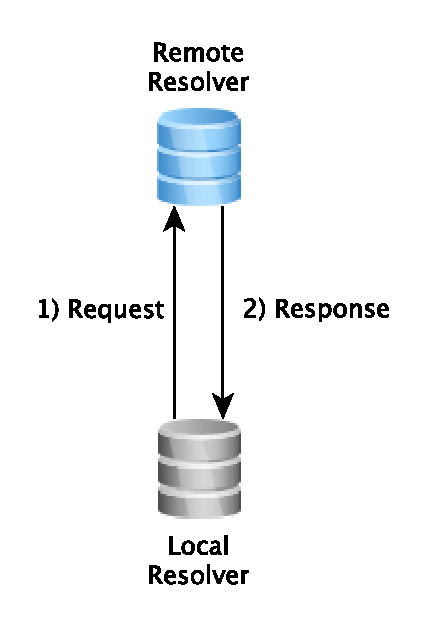
\includegraphics[width=.6\columnwidth]{figures/after}
%      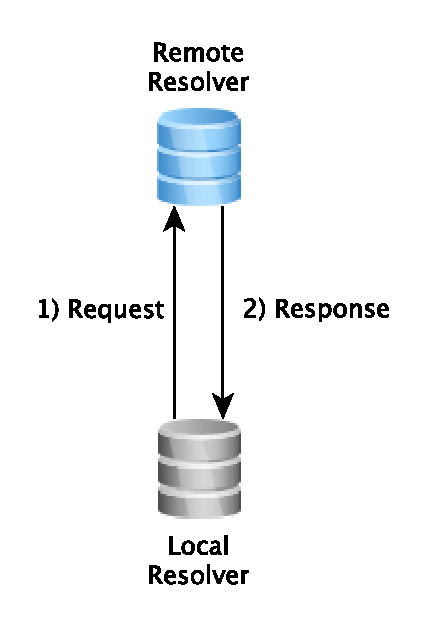
\includegraphics[width=.6\columnwidth]{figures/after}
%      \caption{\textbf{After}}
%      \label{fig:after}
%    \end{subfigure}
%    \caption{For DNSSEC, verifying the DNSSEC signature chain requires many requests to many different remote servers. With our proposal, there is no additional verification strictly necessary.}
%    \label{fig:before-and-after}
%  \end{minipage}
%\end{figure}  





\section{Proposal}\label{sec:proposal}

We want to reduce the overhead of the certificate chain verification in DNSSEC.
By reducing the number of signature  verifications that are necessary, we reduce
the majority of overhead costs --- queries, bandwidth, and latency --- to near 
zero. \footnote{DNS responses will remain larger due to the addition of  DNSSEC
signature records which are not present in vanilla DNS.}

To do this, we propose using a long-lived, mutually authenticated TLS connection
between resolvers. With mutual authentication, both resolvers can provably show
that they know who they are talking to. If one resolver trusts what the  other 
resolver says, there should not be a need to re-verify the DNSSEC signature
chain. This reduces the overhead to near zero, as there will only be
DNSSEC verification if the remote resolver does not use our proposed trust
mechanism.

There are two questions that are still left to answer. First, how do we know a
DNSSEC resolver is trustworthy? Second, what if the remote resolver has been 
compromised? These are both variants of the same question: How can we show that
the remote resolver is trustworthy?
To solve this final problem, we have two solutions. The first solution is
entirely internal to the resolver trying to establish trust: verifying a 
portion of the DNS responses from the remote resolver. If the local resolver 
verifies, say, 5\% of all responses for validity, it probabilistically confirms 
that the remote resolver is trustworthy. This will reduce the amount of extra 
work (over traditional DNS) by near 95\%. This number can be adjusted up or 
down, depending on level of trust (or paranoia) that the administrator has in
the operator of the remote resolver. One automated method would be to perform
DNSSEC certificate chain verification on all responses at the beginning of a 
session, then slowly tapering down to a much lower level of only a few percent
after a while without issue.

The second solution involves using a reputation system, which are typically 
external to a domain. If a large enough number of resolvers use the 
probabilistic system described above, a reputation system could be established 
by aggregating whether or not a particular resolver has ``lied'' and provided 
incorrect DNSSEC responses. 
Other resolvers that use the reputation system could tailor their 
verification strategy based on reputation of the remote resolver. 
For instance, one resolver that cares very strongly about 
security could verify any and all responses from resolvers that it uses, and 
report on the other resolvers' trustworthiness.
A more security lax resolver may verify 50\% of responses from resolvers with a
``bad'' reputation, but only 5\% of responses from those with a ``good'' 
reputation, just to keep them honest and to report back to the reputation 
system. 

These are two \emph{classes} of solutions. There can be  multiple different 
different versions, each tailored to different behaviors of malicious resolvers.
Finding a middle ground to handle different types of behavior well, while 
reducing DNSSEC signature verification overhead is the main challenge.

There is a certificate chain verification cost when establishing a TLS 
connection, but it is a one-time cost, rather the constant recurrent cost like 
DNSSEC signature verifications. The overhead reductions can be seen in 
Table~\ref{table:costs}. The overhead reduction is primarily dependent on how 
much DNSSEC signature verification an administrator wants to use. It is also 
dependent on how long lived the TLS connections are. Perfect reduction is not 
possible while still maintaining reasonable security, if only  because multiple 
connections may be needed for different remote resolvers.

\begin{table}
  \centering
  \begin{tabular}{|l|l|l|}
    \hline
    & \textbf{PKI Ops.} & \begin{tabular}{l}
      \textbf{Additional} \\ 
      \textbf{Queries} \end{tabular} \\
    \hline
    \textbf{Traditional DNS} & 0 & 0 \\
    \hline
    \textbf{DNSSEC} & $N$ & $\sim10N$ \\
    \hline
    \textbf{With Alt. Trust} & 1 & 0 \\
    \hline
    \textbf{5\% Verified Alt. Trust} & $1+\sim0.05N$ & $\sim0.5N$ \\
    \hline
  \end{tabular}
  \caption{Expected overhead versus traditional DNS. \emph{Alt. Trust} refers to
    our proposed solution without any additional verification. 
    \emph{5\% Verified Alt. Trust} refers to verifying 5\% of ``trusted'' 
    responses from other DNS resolver. Transfers are estimated as a factor of 10
    over traditional DNS.\cite{huston2013}}
  \label{table:costs}
\end{table}




\balance\section{Conclusion and Future Work}\label{sec:conclusion}

We have proposed using a long-lived, mutually authenticated TLS connection
between two DNSSEC-enabled resolvers as an alternative source of trust in order
to reduce the overhead of performing DNSSEC signature  verification operations.
We have shown that, while having potential security issues, we can mitigate 
compromised machines by probabilistically verifying DNSSEC responses to build 
trust.

This method is similar to how stub resolvers (\ie, hosts) maintain DNSSEC 
guarantees. RFC 4033 specifically suggests using IPSEC to maintain security
between the stub resolver and the recursive resolver.\cite{rfc4033} Using TLS
provides similar guarantees. Additionally, this method expands the ongoing work
of the DNS privacy working group within the IETF from not only stub-to-recursive
resolver connections, but between recursive resolvers.

As the security of this proposal hinges on the trustworthiness of the DNS 
resolver that a TLS connection is established with, our first course of action 
is to create and simulate our proposed solutions for establishing trust. 
While some scenarios could be represented by a Bayesian model, others lend 
themselves to simulation. In particular, as the probabilities for verification 
change based on previous input, simulation is easier for determining whether a
a particular strategy for verification is effective.

Developing models for malicious resolver behavior and strategies for countering


These
need not involve actual DNS resolution, rather these can be simulated in a much
simpler environment. Some scenarios may be modeled using Bayes rules, but only
if probabilities are known and consistent. Other scenarios have ``moving 
parts'' --- such as changes in the probability of verification --- where 
simulation is more appropriate. Finally, different behaviors of a malicious 
resolver can be more easily simulated, such as a resolver that only `lies' about
one particular domain and provides valid results for all others. Different 
strategies may be necessary for establishing trust 

Further, we plan on implementing this scheme on an existing 
DNSSEC-enabled resolver, such as BIND or Unbound. 
We will then test this method for both
practicality --- verifying that there is a processing and network  cost savings 
compared to verifying all DNSSEC messages --- and security --- by `compromising'
one resolver and seeing the response from the non-compromised resolver, 
specifically how long it takes to find that the one resolver is ``lying''.

Further, we see this alternative model of trust could be used in other 
scenarios. For instance, the various security schemes surrounding BGP (BGPSEC, 
S-BGP, RPKI, etc.) all rely on PKI verification, much like DNSSEC. This 
technique could be applied for similar savings with potentially different 
criteria for verification, such as for any prefixes being announced by 
autonomous systems (ASes) known to host malware. 

This is not a method for absolute security, like DNSSEC is aiming for, rather 
this is for practical security with low overhead. It can be used to alleviate
scalability concerns particularly on a closed network where all DNS resolvers are
controlled by the same organization. It is also useful for an organization that
has less strict security requirements but wants to benefit from DNSSEC with 
lower cost.

\label{lastpage}

\end{sloppypar}

%\vspace{-0.1in}
%\section*{Acknowledgments}
% Comments for people we need to acknowledge in the final version.

%\pagebreak

\small
%\setlength{\bibsep}{0pt}
\setlength{\parskip}{-1pt}
\setlength{\itemsep}{-1pt}
% \footnotesize % SPACE
\balance\bibliography{paper}
\bibliographystyle{abbrv}
%\bibliographystyle{abbrvnat_noaddr} % SPACE
%\theendnotes % ENDNOTES
}{% onlyAbstract
}

\end{document}

%%%%%%%%%%%%%%%%%%%%  END OF DOCUMENT  %%%%%%%%%%%%%%%%%%%%
